\documentclass[11.5pt]{article}
\usepackage[margin=1in]{geometry}
\usepackage{hyperref}
\usepackage{graphicx}
\usepackage{subcaption}



\title{Recognize Animation Characters with Machine Learning}

\author{Xin Guan, Ziqian Ge}

\date{}

\begin{document}

\maketitle

\abstract
Please provide a brief abstract of your project.

\vspace{2mm}
\section{Introduction}
As the fandom community of animation grows, a large number of fan-arts made by non-official illustrators began to show up and gradually became an significant part of the community.
Fan-arts spread on the internet are often not labeled or are hard for people, especially those who are new to the community, to recognize the illustrating character, since many anime characters shares similar characteristics and different illustrators may shift some of the features base on their own taste.\\ \\
Untagged illustrations would make some trouble for animation community members. 
Large number of 'Who is she/he' questions are emerging on social networks plantforms like Twitter, 2Chan and Bilibili. 
Even some video makers are making videos on answering those questions. 
On the other hand, within the machine learning community, if anyone is trying to make a illustration suggestion system based on the features or characteristics of anime characters, or trying to use GAN (Generative Adversarial Network) to generate fake anime illustrations, they might have to tag those pictures manually.\\ \\
Automatic character recognizing would then make some differences when one is facing a large set of untagged illustrations or would like to add/optimize tags based on character, for example, a character may be bounded to specific tags, like blond, green-eye, sword, armored, etc.\\ \\
This project is aiming to use machine learning techniques to automatically recognize characters in illustrations, based on their faces. We are mainly focusing on characters from japanese styled mangas and aminations. This project is making use of a variety of classification models including models like logistic regression classifier, random forest classifier and support vector machine and neural networks.\\ \\
In order to make it possible to train non-neural-network models, we performed feature extraction techniques on images during the preprocessing stage. The first strategy is extracting the texture, color and shape of the image contents and then flattern those features to an vector for the models to lean. The second strategy is extracting features using the output of the last layer of pre-trained ResNet[] as the image features and train them on non-neural-network models.\\ \\
In this project, we did hyperparameter tunning on a rather small dataset that is collected manually by us and then train the model on the whole dataset which consists of ours and Nagadomi’s anime face character dataset[]. Neural network performed best with a recognition rate of 90\%. Support vector machine was the best model among non-neural-network models with ResNet extracted features. However, our first strategy leads to rather poor accuracy rate on all models (about 20\% accurate rate on 178 classes). 


\section{Technical Approach}
Please describe the techniques you have used in order to address the problem.
Describe in detail the classification/regression/other techniques you have used in order to tackle the problem.

We did some initial data filtering on Nagadomi's anime face character dataset and added some data collected by ourselves.
The original dataset contains a lot of falsely labeled images, some differently labeled images that are actually the same character, a lot of images that cannot be recognized even by human, and a lot of characters does not contain sufficient amount of data, i.e.\ some characters has less than 100 images.
Bad images like ones described above were removed from our dataset manually.\\ \\
\begin{figure}[h!]
    \begin{subfigure}[b]{0.4\linewidth}
        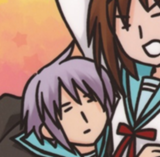
\includegraphics{../data_set/moeimouto-faces/007_nagato_yuki/face_145_303_113.png}
        \caption{Nagato Yuki}
    \end{subfigure}
    \begin{subfigure}[b]{0.4\linewidth}
        
\includegraphics{../data_set/moeimouto-faces/007_nagato_yuki/face_235_235_128.png}
        \caption{Nagato Yuki}
    \end{subfigure}
    \caption{Comparison between a bad image and a good image}
\end{figure}
\begin{figure}[h!]
    \begin{subfigure}[b]{0.4\linewidth}
        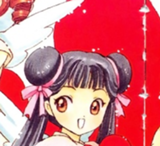
\includegraphics{../data_set/moeimouto-faces/074_daidouji_tomoyo/face_795_301_69.png}
        \caption{Meirin Ri labeled as Daidouji Tomoyo}
    \end{subfigure}
    \begin{subfigure}[b]{0.4\linewidth}
        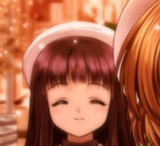
\includegraphics{../data_set/moeimouto-faces/074_daidouji_tomoyo/face_451_275_121.png}
        \caption{Real Daidouji Tomoyo}
    \end{subfigure}
    \caption{The character on the left, Meirin Ri is falsely labeled as Daidouji Tomoyo}
\end{figure}

There are a total of 173 characters, and it was impracticable to train our models and tune hyper-parameters using all of our data, we decide to pick some characters each with over 100 images to make subset of the total dataset to tune hyper-parameters.\\ \\
We have made our classification in three major directions: traditional models, neural network (ResNet), and combining traditional models and neural network.\\ \\
For traditional models approach, we have trained logistic regression classifier, K neighbors classifier, decision tree classifier, random forest classifier, Gaussian Naive Bayes classifier, and support vector machine classifier using scikit-learn to tune hyper-parameters on the subset described above.
The classification result using all of our data was produced using the model performing the best in the subset after all hyper-parameter was tuned.\\ \\
For neural networks approach, we chose ResNet, which was implemented in PyTorch, to be our neural network model.
We have trained ResNets with different number of layers, 18 layers (ResNet18), 34 layers (ResNet34), 50 layers (ResNet50), 101 layers (ResNet 101) on the same subset that was used in hyper-parameter tuning process of traditional models to find the network with number of layers performing the best.
The classification result using all of our data was also produced using the network performing the best in the subset.\\ \\
For the combination of traditional models and neural network approach, we decided to train traditional models using the results from the neural network that was chosen in the neural networks approach, so that the ResNet would work as a feature extraction method for traditional models.
Hyper-parameters was tuned using the same subset of data in the previous approaches, and the result using all of our data would also be produced after hyper-parameters was tuned.\\ \\
In details of traditional models, models was actually trained using features extracted from the raw RGB data.
This feature extraction process was a direct combination of HuMoments (implemented in OpenCV), Haralick features (implemented in mahotas), and color histogram (implemented in OpenCV), by plugging them into each other.
The order of feature extraction we chose was: HuMoments $\rightarrow$ Haralick $\rightarrow$ color histogram.\\ \\
For tuning hyper-parameters of logistic regression classifier, logistic regression models with or without regularization functions and different regularization strength (C in scikit-learn) was trained to find the best penalty function and the value of regularization strength.
Since we chose to use "lbfgs" solver in scikit-learn, we can only use l2-norm in penalization, or use no regularization.
The regularization strength, C, was tested with floats ranging from $0.1$ to $10.0$ to find the best value.\\ \\
For tuning hyper-parameters of K neighbors classifier, we tried out different values of $k$, ranging from $1$ to $30$ to find the best value of $k$.\\ \\
For tuning random forest classifier, we tried forests with different loss function, Gini impurity function and Information Entropy function, and different number of estimators to find the best value of them.\\ \\
For tuning support vector machine classifier, we tried different kernels, linear, polynomial, rbf, and sigmoid kernels to find the best kernel among them.
For polynomial kernel, we have also tried and tested different degree of polynomial kernel, ranging from $1$ to $20$, to find the best degree.
The regularization strength, C, was also tested with floats ranging from $1$ to $30.0$ to find the best value.\\ \\
The same process of hyper-parameter tuning was also performed in the ResNet-traditional combined approach, as the best values in different approaches are not guaranteed to be the same.

\section{Experimental Results}
Describe the datasets used for your experiments. Be precise in describing all information about the datasets, including, classes, number of samples per class, features used to represent data, and all pre/post processing of the datasets.\\
Describe the details about the implementation of each algorithm, e.g., how you perform training, validation, testing, values of the hyperparameters and your methods for hyperparameter tuning, training/validation/testing error on the dataset, and all useful plots/tables that help to better interpret your results and your work.\\ \\
In this project, we are going through following working pipeline. Firstly, we manually clean the Nagadomi's Anime Face Character Dataset and generate our own dataset with better image quality and mordern animation characters. Then, we perform image preprocessing and feature extractions to generate three union of data: color-texture-shape information, resnet-processed information and normalized RGB information. Then we design different models according to these unions of data. According to our models, we do hyperparameter tunning on the self-collected dataset and then train the model with the optimized hyperparameter on the whole dataset and evaluate the prediction result. Following are the detailed description of each step in the working pipeline.

\begin{enumerate}
    \item \textbf{Dataset Overview}
        \begin{itemize}
            \item \textbf{Self-collected Dataset}
            \item \textbf{Nagadomi’s Anime Face Character Dataset}
        \end{itemize}
    \item \textbf{Non-Neural-Network Models}
        \begin{itemize}
            \item \textbf{Data Pre-processing and Feature Extracting}
            \item \textbf{Hyperparameter Tunning}
            \item \textbf{Prediction Result}
        \end{itemize}
    \item \textbf{Neural-Network Model}
        \begin{itemize}
            \item \textbf{Data Pre-processing}
            \item \textbf{Hyperparameter}
            \item \textbf{Prediction Result}
        \end{itemize}
\end{enumerate}

\section{Participants Contribution}
Please list the name of the participants. For each participant explain in details the role he/she played in the project: explain which methods was implemented by which member, which dataset was processed by which member, which experimental results were generated by which members, etc.

\vspace{10mm}
** Please do not change the size of the fonts.

** Please note that your submission must be at most 7 pages long, excluding references.

\end{document}
